\begin{cn}
\textgreek{Τὰ ἐφαρμόζοντα ἀλλήλοις ἴσα ἐστίν.} (Ta epharmozonta allēlois isa estin) \\
Things which coincide with one another are equal to one another.
\end{cn}

\begin{figure}[H]
\centering
\begin{subfigure}{0.3\textwidth}
\centering
\begin{tikzpicture}
\tkzDefPoint(0,0){A}
\tkzDefPoint(3,0){B}
\tkzDefPoint(1.5,2){C}
\tkzDrawPolygon[fill=red!55](A,B,C)
\tkzCentroid(A,B,C)  				\tkzGetPoint{D}
\tkzLabelPoint[above](D){$\alpha$}
\end{tikzpicture}
\caption{Triangle $\alpha$}
\end{subfigure}%
\begin{subfigure}{0.3\textwidth}
\centering
\begin{tikzpicture}
\tkzDefPoint(0,0){A}
\tkzDefPoint(3,0){B}
\tkzDefPoint(1.5,2){C}
\tkzDrawPolygon[fill=green!55](A,B,C)
\tkzCentroid(A,B,C)  				\tkzGetPoint{D}
\tkzLabelPoint[above](D){$\beta$}
\end{tikzpicture}
\caption{Triangle $\beta$}
\end{subfigure}
\begin{subfigure}{0.3\textwidth}
\centering
\begin{tikzpicture}
\tkzDefPoint(0,0){A}
\tkzDefPoint(3,0){B}
\tkzDefPoint(1.5,2){C}
\tkzDrawPolygon(A,B,C)
\begin{scope}
    \tkzClipPolygon(A,B,C)
    \path[pattern=north west lines, pattern color=red] (A) -- (B) -- (C) -- cycle;
    \path[pattern=north east lines, pattern color=green] (A) -- (B) -- (C) -- cycle;
\end{scope}
\end{tikzpicture}
\sidecaption[c][-2cm]{Superimposition showing $\alpha$ coincides exactly with $\beta$}
\end{subfigure}
\caption{Illustration of Common Notion 4: Geometric coincidence implies equality.}
\end{figure}

As $\alpha$ fits exactly on top of $\beta$ without any overlap, this demonstrates that $\alpha \cong \beta$, showing geometric congruence as per Common Notion 4.

\textbf{Linguistic Analysis:}
The term \textgreek{εφαρμόζω} (epharmozō), meaning "to fit exactly" or "to coincide," is crucial in understanding the precision of Euclidean geometry. This term is used in different voices to express variations in meaning:
\begin{enumerate}
\item \textbf{Passive Voice:} \textgreek{εφαρμόζεσθαι} (epharmozesthai) - "to be applied to," suggesting a possible but not guaranteed exact fit.
\item \textbf{Active Voice:} \textgreek{εφαρμόζω} (epharmozō) - implies a perfect alignment without overhang or shortfall.
\end{enumerate}

Furthermore, the prepositions and cases used with \textgreek{εφαρμόζω} affect its interpretation:
\begin{itemize}
\item \textbf{With \textgreek{πρός} (pros) and Accusative:} Indicates dynamic motion towards alignment.
\item \textbf{With Dative:} Implies a static, existing state of application, common in the writings of Pappus.
\end{itemize}

These subtleties enhance our understanding of Euclid's methods and the precise nature of geometric proofs in the \textit{Elements}.

\clearpage